\section{Experiments}

\subsection{Simulating MPC}

\begin{figure}[H]
\centering
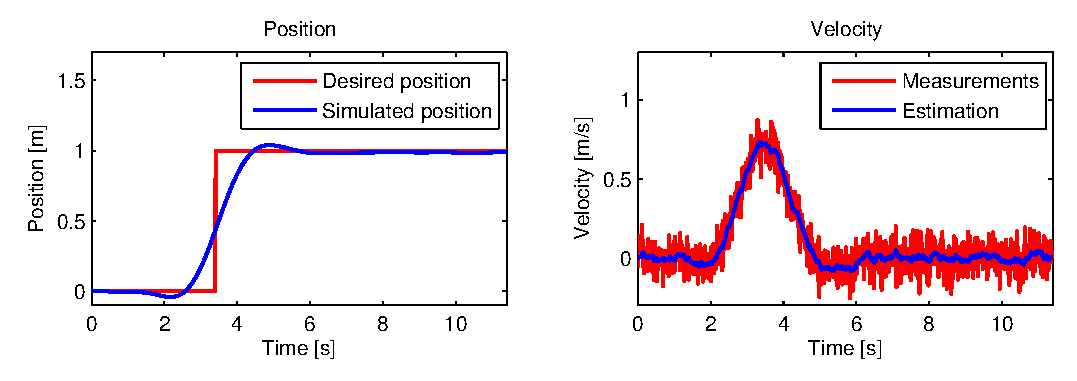
\includegraphics[width=0.99\textwidth]{fig/simulation1.eps}
\caption{Simulating position step response without the input governor.}
\label{fig:simulation_step_no_governor}
\end{figure}

\begin{figure}[H]
\centering
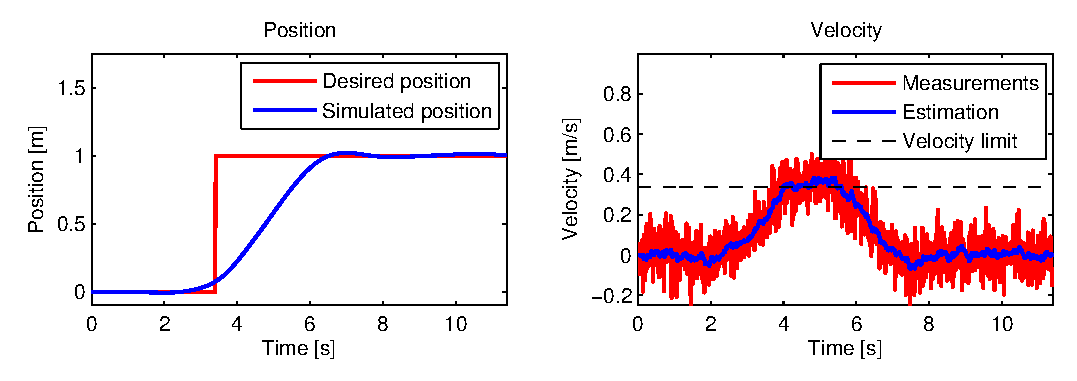
\includegraphics[width=0.99\textwidth]{fig/simulation2.eps}
\caption{Simulating position step response with the input governor.}
\label{fig:simulation_step_governor}
\end{figure}

\begin{figure}[H]
\centering
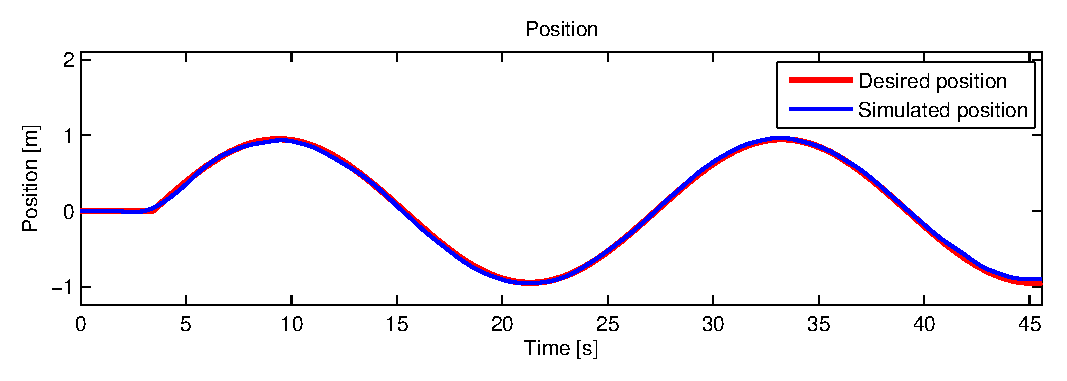
\includegraphics[width=0.99\textwidth]{fig/simulation3.eps}
\caption{Simulating trajectory of feasible sine trajectory.}
\label{fig:simulation_step_governor}
\end{figure}

\begin{figure}[H]
\centering
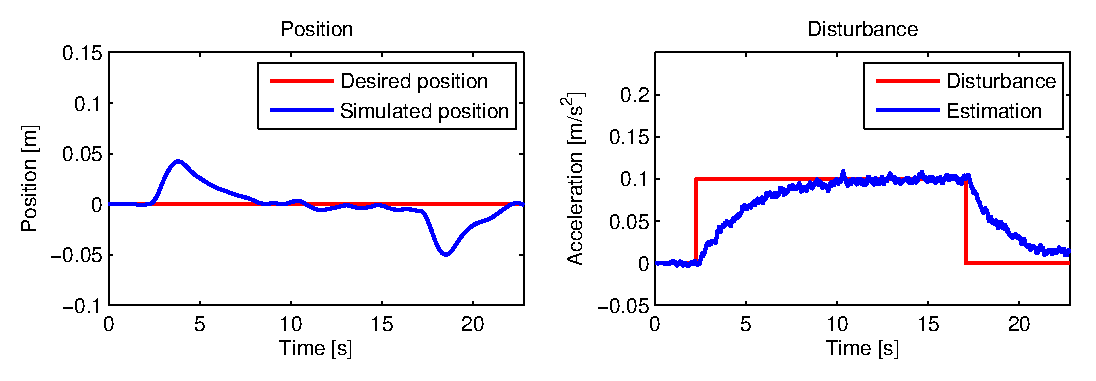
\includegraphics[width=0.99\textwidth]{fig/simulation4.eps}
\caption{Simulating of disturbance rejection.}
\label{fig:simulation_step_governor}
\end{figure}

\subsection{Static trajectory performance}

\subsection{Tracking dynamic trajectory}
\label{cap:dynamic_trajectory_tracking}

\begin{figure}[h]
\centering
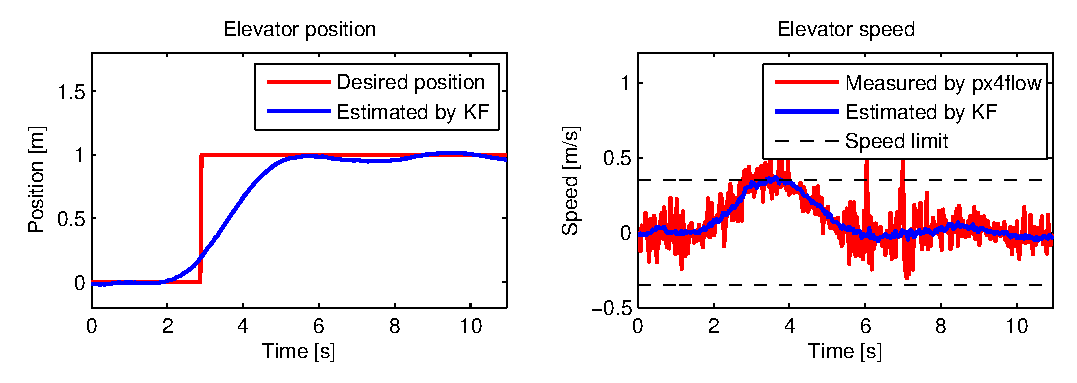
\includegraphics[width=0.99\textwidth]{fig/experiment2_step.eps}
\caption{Experiment with step response. The trajectory was not precomputed --- the step reference occurred suddenly, thus the controller was not proactive.}
\label{fig:experiment_sine_1}
\end{figure}

\begin{figure}[H]
\centering
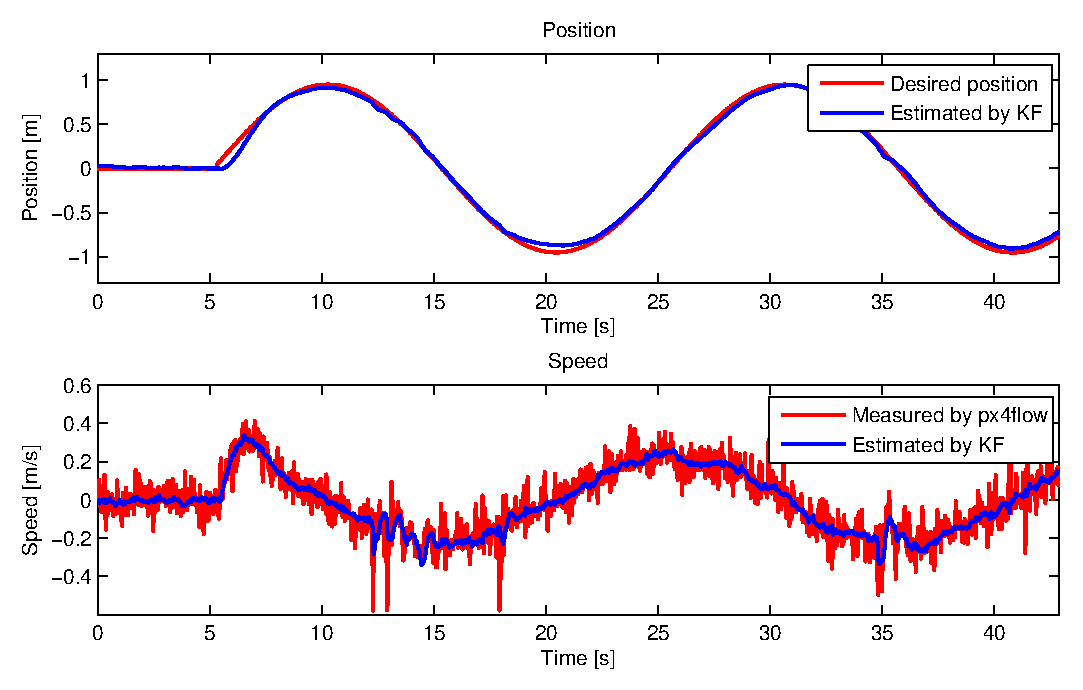
\includegraphics[width=0.99\textwidth]{fig/experiment1_sine.eps}
\caption{Experiment with tracking circular trajectory. Figures show position and velocity in single axis.}
\label{fig:experiment_sine_1}
\end{figure}

\subsection{Disturbance rejection}

\subsubsection{Persistent disturbance}

\begin{figure}[H]
\centering
	\begin{tikzpicture}
		\node[anchor=south west,inner sep=0] (a) at (0,0) {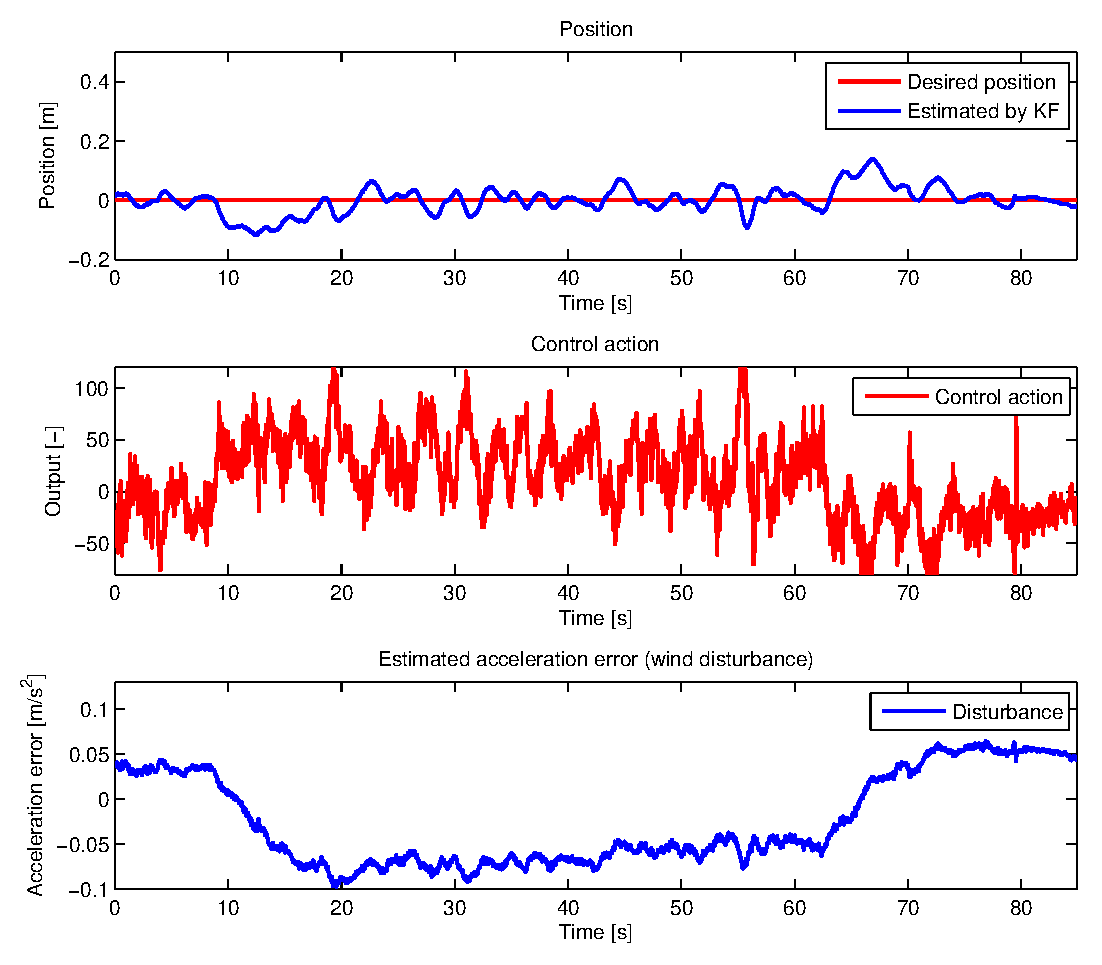
\includegraphics[width=\textwidth]{fig/experiment3_steady_disturbance.eps}};
		\begin{scope}[x={(a.south east)},y={(a.north west)}]

		%\draw[help lines,xstep=.1,ystep=.1] (0,0) grid (1,1);	
		
%        \draw[white,ultra thick,rounded corners] (0.55,0.50) rectangle (0.7,0.7);
%        \draw (0.58,0.655) node [text=white] {\textbf{1}};
        

		\draw[-latex] (0.2,0.9) -- (0.2,0.81);    
		\node[] at (0.25,0.92) {Disturbance started};    
		
		\draw[-latex] (0.75,0.9) -- (0.795,0.81);    
		\node[] at (0.65,0.92) {Disturbance went off};  
        
    \end{scope}
	\end{tikzpicture}
\caption{Experiment with tracking constant setpoint while being under the influence of wind.}
\label{fig:experiment_steady_wind}
\end{figure}

\subsubsection{Momentary disturbances}
\label{cap:momentary_disturbances}

\subsection{Summary and comparison with previous work}